
\label{sec:calibration}
\
The parameter values which represent biological process ($\alpha, \gamma_{I}, \gamma_{D}, \delta_{1}, \delta_{2}$) or social custom ($\gamma_{F}$) were discovered in many sources [reference], while the parameters which represent social behavior ($\mathcal{P}=\{\beta_{I}, \beta_{H}, \beta_{F}, \gamma_{H}, \theta\}$) are site-dependent and unknown. $\gamma_{DH}$ and $\gamma_{IH}$ are also unknown, but we assume that they are dependent on other variables ($1/\gamma_{DH}$=$1/\gamma_{D}$-$1/\gamma_{H}$ and $1/\gamma_{IH}$=$1/\gamma_{I}$-$1/\gamma_{H}$). In this chapter, we calibrated $\mathcal{P}$ based on our systematic model (equation link) and the data of cumulative death in Liberia from March 2014 to July 2015 (reference).
\subsection{Bayesian calibration framework}
Using Bayesian calibration methodology, we calibrate the unknown parameters ($\mathcal{P}$). The prior distribution of $\mathcal{P}$ is a uniform distribution which ranges are determined based on numerical exploration and previous researches [references] (Table). \\

\begin{table}[ht]
\caption{Range of the prior parameter space} % title of Table
\centering % used for centering table
\begin{tabular}{c c c c c}
\hline\hline %inserts double horizontal lines
$\beta_{I}$ & $\beta_{H}$ & $\beta_{F}$ & $\gamma_{H}$ & $\theta$ \\ [0.5ex]
\hline % inserts single horizontal line
$(0,0.5)$ & $(0,0.5)$ & $(0,1)$ & $(2,7)$ & $(0,0.5)$ \\ [0.5ex]
\hline
\end{tabular}
\label{tab:Prior Ranges}
\end{table}


To each random choice ($\mathcal{P}_0$) from the prior distribution, we assign likelihood weight by comparing the real world data ($\mathcal{D}_R$) and data simulated with $\mathcal{P}_0$ ($\mathcal{D}_S$). Multiple choices of parameters and their weights will eventually construct the posterior distribution of $\mathcal{P}$. In this methodology, we provide multiple likely parameter sets, rather than a single best fit. Detailed description on the calibration procedure is:\\

Step 1) Choose a random $\mathcal{P}_0$ from the prior distribution

Step 2) Solve our deterministic system (equation link) with $\mathcal{P}_0$ and given initial value $\{S_0,E_0,I_0,F_0,D_0,R_0\}$, then evaluate $\mathcal{D}_S=\{D(t_i)\}$ for all dates $\{t_i\}$ corresponding to the cumulative death data ($\mathcal{D}_R$).

Step 3) Evaluate likelihood of $\mathcal{P}_0$: $Exp[-Norm(\mathcal{D}_R-\mathcal{D}_S)/Norm(\mathcal{D}_R)]$

\emph{Repeat Step 1-3 multiple times and make large number of {parameter + likelihood} ensembles. Generate posterior distribution with them.}

\subsection{Results and validation}
For the calibration of before intervention parameters, we used the data for 176 days (March 14 to September 14), and initial value $\{S_0,E_0,I_0,F_0,D_0,R_0\}$=$\{10^6-1,0,1,0,0,0\}$ assuming that initial outbreak started from a single infected person in a million population. The calibration of after intervention parameters is based on the data for 306 days (September 14 to July 15), and initial value $\{S[176],E[176],I[176],F[176],D[176],R[176]\}$ which are evaluated from calibrated mean $\mathcal{P}$ for pre intervention. 10000 random samples were used in each calibration. Calibration results and validation are shown in (table) and (figure).\\
Based on our calibration, the intervention reduce the basic reproduction number of Ebola in Liberia from 1.99 to 0.787, using the formula in (reference). As a result, disease spread is terminated after infecting 0.84\% of total population with 0.49\% decrease in population, otherwise 92.7\% are infected and population decreases by 53.5\%.\\


\begin{table}[ht]
\caption{Model Parameters for Ebola Epidemic in Liberia Before and After the International Intervention. Calibrated parameters are written in bold font, and posterior means and standard deviations in parenthesis are notated.} % title of Table
\centering % used for centering table
\begin{tabular}{c c c }
\hline\hline %inserts double horizontal lines
Parameter & Liberia Before Intervention  & Liberia After Intervention \\ [0.5ex]
 & (Mar/14 to Sept/14) &  (Sept/14 to Jul/15) \\ [0.5ex] % inserts table
% inserts table
%heading
\hline % inserts single horizontal line
\bf {Contact Rate, Community  ($\bf{\beta_{I}}$) }& \bf{0.148 (0.0953)} & \bf{0.0446 (0.338)}  \\
\bf Contact Rate, Hospital  ($\beta_{H}$) &\bf 0.235 (0.143)& \bf 0.0877 (0.563) \\
\bf Contact Rate, Funeral  ($\beta_{F}$) & \bf 0.465 (0.287)& \bf 0.283 (0.208) \\
Incubation Period (${1}/{\alpha}$) & 11 days & 11 days  \\
\bf Time until Hospitalization (${1}/{\gamma_{H}}$) &\bf 4.49 (1.44) days & \bf 4.63 (1.43) days  \\
Time froml Hospitalization to Death (${1}/{\gamma_{DH}}$) & 3.51 days & 3.51 days  \\
Duration of Traditional Funeral (${1}/{\gamma_{F}}$) & 2.00 days & 2.00 days  \\
Duration of Infection (${1}/{\gamma_{I}}$) & 10.00 days & 10.00 days  \\
Time from Infection to Death (${1}/{\gamma_{D}}$) & 8.00 days & 8.00 days  \\
Time from Hospitalization to Recovery (${1}/{\gamma_{IH}}$) & 5.51 days & 5.51 days  \\
\bf Probablity a Case is Hospitalized ($\theta$) & \bf 0.248 (0.142) & \bf 0.233 (0.145) \\
Case Fatality Rate, Unhospitalized ($\delta_{1}$) & 0.500  & 0.500  \\
Case Fatality Rate, Hospitalized ($\delta_{2}$) & 0.500 & 0.500 \\ [1ex]
\hline
\end{tabular}
\label{tab:parameters}
\end{table}


\begin{figure}
  \centering
  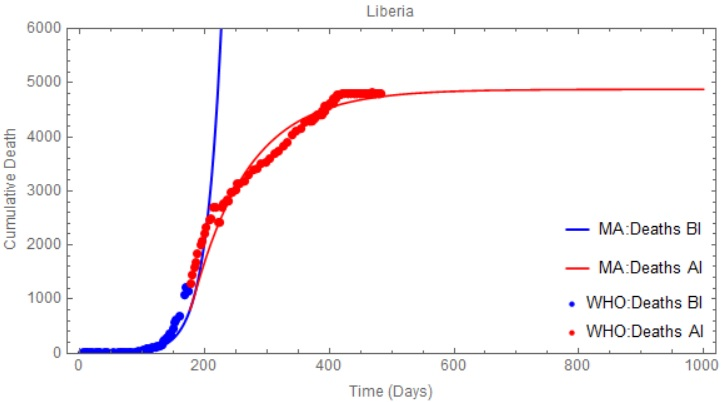
\includegraphics[width=0.7\textwidth]{CumulativeDeathMathematica}
  \caption{write caption here}
\label{fig:Validation of calibration. Dots represent cumulative death data and the lines represent simulation based on mean posterior parameters. (Blue) - pre intervention and (red) - post treatment.}
\end{figure}
